% !TeX program = pdflatex
%==============================================================================
%  Aula 03 --- Seleção de Modelos e Validação Cruzada
%  VERSÃO DO ALUNO: texto para leitura autônoma, fora da sala.
%  (O roteiro de sala correspondente é "03 Validacao Cruzada.tex".)
%==============================================================================
\documentclass[11pt,a4paper]{article}
\usepackage[aluno]{../../recursos/latex/estilo-notas}

\title{}
\date{}

\begin{document}
\cabecalhoaula{03}{Seleção de Modelos e Validação Cruzada}{AME §1.4--1.5; ISLP cap.~5}

%==============================================================================
\section*{O que você vai aprender}
%==============================================================================
Ao final desta aula você deve ser capaz de:
\begin{itemize}[leftmargin=1.4cm]
  \item explicar por que o erro de treino é um estimador \emph{otimista} do risco;
  \item descrever \emph{data splitting} (treino/validação) e estimar o risco com a
        parte de validação;
  \item definir \emph{validação cruzada} LOOCV e $k$-dobras e relacioná-las;
  \item discutir o balanço viés--variância \emph{na própria estimativa do risco} e
        a escolha de $k$;
  \item usar a validação cruzada para \textbf{selecionar hiperparâmetros} sem
        vazamento;
  \item descrever o \emph{bootstrap} para quantificar incerteza de uma estimativa.
\end{itemize}

\noindent
Esta é a aula \emph{operacional} mais importante do curso. Nas Aulas~01 e~02
apareceram hiperparâmetros --- o grau do polinômio, o $\lambda$ do Lasso --- e nos
dois casos a resposta para ``como escolher?'' foi ``na Aula~03''. Chegamos nela. A
mesma ferramenta vai escolher o $k$ do KNN, a profundidade da árvore, o $C$ da SVM.
Comece pela pergunta:

\begin{center}\itshape
  se eu ajustar um polinômio de grau 50 a 50 pontos, qual o erro no treino?\\
  e isso quer dizer que é um bom modelo?
\end{center}

\noindent
O erro é \emph{exatamente zero} --- 51 parâmetros passam por 50 pontos sem esforço
--- e o modelo é péssimo. Um critério de qualidade que dá nota máxima ao pior modelo
possível não serve como critério. Precisamos de outro.

%==============================================================================
\section{O problema: estimar o risco}
%==============================================================================
Da Aula~01, o risco de uma função de predição $g$ é
$\risco(g)=\E[L(Y,g(\X))]$, esperança sobre uma observação \emph{nova}. Para
\emph{selecionar} um modelo (escolher entre candidatos $g\in\mathcal{G}$, ou
escolher um hiperparâmetro) precisamos comparar riscos --- mas $\risco(g)$ é
desconhecido porque depende de $P$. Logo, \textbf{tudo se resume a estimar bem o
risco}.

\subsection{Por que não usar o erro de treino?}
O candidato ingênuo é o \emph{erro quadrático médio no treino} (risco empírico):
\begin{equation}\label{eq:eqm}
  \mathrm{EQM}(g) = \frac1n \sum_{i=1}^n \big(Y_i - g(\X_i)\big)^2 .
\end{equation}
O problema: $g$ foi \emph{escolhida para ajustar exatamente esses pontos}. O
EQM\eqref{eq:eqm} é um estimador \textbf{otimista} (enviesado para baixo) de
$\risco(g)$, e esse viés --- o \emph{otimismo} --- cresce com a complexidade do
modelo.

\begin{atencao}[dois ``vieses'' diferentes, e eles andam em sentidos opostos]
A palavra \emph{viés} acabou de mudar de sentido, e vale parar um instante, porque
a Aula~01 ensinou o outro:
\begin{itemize}[leftmargin=1.4cm,nosep]
  \item \textbf{o viés do modelo}, da decomposição viés--variância da Aula~01:
        $\E_\Dados[\rhat(\x_0)]-r(\x_0)$, o quanto o método erra o alvo $r$. Esse
        \textbf{cai} com a complexidade --- é a curva que desaba a partir do
        grau~5 na figura da decomposição;
  \item \textbf{o viés do EQM de treino como estimador do risco}:
        $\E[\mathrm{EQM}(g)]-\risco(g)$, o quanto a \emph{régua} mente. Esse
        \textbf{cresce} com a complexidade, e é dele que a frase acima fala.
\end{itemize}
São objetos de níveis diferentes: um é o erro do modelo, o outro é o erro da
\emph{medida} do erro do modelo --- e não há contradição em o mesmo modelo ter os
dois. O grau~49 da §3 da \texttt{Aula prática 03} é o caso extremo: erro de treino
$0{,}1029$, \emph{menor} que o $0{,}3580$ do grau~5, e risco $2{,}5\times 10^{13}$.
Ao subir o grau, o viés do modelo desapareceu e o da régua explodiu junto. É por
isso que o erro de treino não pode arbitrar entre modelos de complexidades
diferentes: quanto mais flexível o candidato, mais a régua o favorece.
\end{atencao}

\begin{atencao}
Levado ao extremo, minimizar o erro de treino leva ao superajuste perfeito: um
modelo flexível o bastante \emph{interpola} os dados (erro de treino zero, em
aritmética exata --- ver a §3 da \texttt{Aula prática 03} para o que o ponto
flutuante faz com isso) e generaliza pessimamente. \textbf{Nunca} selecione
modelos nem reporte desempenho com o erro de treino.
\end{atencao}

\begin{observacao}
Penalização (AIC, BIC) é uma alternativa: estima-se
$\risco(g)\approx \mathrm{EQM}(g)+P(g)$, com $P(g)$ crescente na complexidade
(p.ex.\ $P(g)\propto p/\widehat\sigma^2$ no AIC). Funciona, mas exige um modelo
probabilístico e contagem de ``parâmetros'' --- nem sempre disponível (KNN,
florestas). A validação cruzada é \emph{agnóstica ao modelo} e por isso a
preferimos.
\end{observacao}

%==============================================================================
\section{Data splitting (conjunto de teste)}
%==============================================================================
A ideia mais simples: separe os dados \emph{aleatoriamente} em treinamento
(p.ex.\ 70\%) e teste (p.ex.\ 30\%):
\[
  \underbrace{(\X_1,Y_1),\dots,(\X_n,Y_n)}_{\text{treinamento}}\;,\;
  \underbrace{(\X_{n+1},Y_{n+1}),\dots,(\X_{n+m},Y_{n+m})}_{\text{teste}}.
\]
Daqui para a frente $n$ é o tamanho do \emph{treinamento} e $m$ o do teste.
Ajuste $g$ \emph{só} no treinamento e estime o risco \emph{só} no teste:
\begin{equation}\label{eq:datasplit}
  \riscohat(g) = \frac{1}{m}\sum_{i=n+1}^{n+m} \big(Y_i - g(\X_i)\big)^2 .
\end{equation}
Como o teste não foi usado para estimar $g$, \eqref{eq:datasplit} é um
estimador \emph{consistente} de $\risco(g)$ pela lei dos grandes números. A
proporção também não é arbitrária: treinar um modelo exige mais informação do que
avaliá-lo, e por isso a fatia maior fica com o treinamento.

\begin{atencao}[o \emph{aleatoriamente} não é decoração]
Se o banco vier ordenado por alguma variável --- por data, por classe, por quem
coletou ---, cortar pelos índices originais produz dois conjuntos que não são
amostras da mesma distribuição, e a estimativa fica sem sentido. Quem montou o banco
pode ter ordenado por um motivo que você desconhece. Em \texttt{scikit-learn} isso é
o \texttt{train\_test\_split(\dots, shuffle=True)}, que já é o padrão --- mas vale
saber por que existe.
\end{atencao}

\begin{atencao}[Limitações do data splitting]
\begin{enumerate}[leftmargin=1.5cm,nosep]
  \item \textbf{Desperdício de dados:} $g$ é treinada com apenas $n$ das $n+m$
        observações que você coletou; com poucos dados isso prejudica o ajuste.
  \item \textbf{Variabilidade:} a estimativa depende da divisão sorteada --- outra
        semente dá outro número. Pode ser instável.
\end{enumerate}
A validação cruzada resolve os dois usando \emph{todo o conjunto de treinamento}
--- e é importante ver o que ela \emph{não} substitui. A divisão treino/teste
continua sendo o primeiro passo, e o teste continua guardado até o fim. O que a
validação cruzada dispensa é um \emph{segundo} corte, o que separaria uma parte do
treino para escolher o modelo: esse papel passa a ser feito pelas dobras, girando
dentro do treino.
\end{atencao}

%==============================================================================
\section{Validação cruzada}
%==============================================================================
\subsection{Leave-one-out (LOOCV)}
Deixe \emph{uma} observação de fora por vez. Seja $g_{-i}$ o modelo ajustado sem a
$i$-ésima observação. O estimador é
\begin{equation}\label{eq:loocv}
  \riscohat_{\text{LOO}}(g) = \frac1n \sum_{i=1}^n \big(Y_i - g_{-i}(\X_i)\big)^2 .
\end{equation}
Cada $Y_i$ é predito por um modelo que \emph{não} o viu. LOOCV é
\emph{aproximadamente não-viesado} para o risco esperado e não tem aleatoriedade de
divisão.

\begin{observacao}[por que ``aproximadamente não-viesado'']\label{obs:loo}
A conta é curta, e o ``aproximadamente'' tem uma causa precisa --- vale ver as
duas. Primeiro uma notação: escreva $\risco_m$ para o risco \emph{esperado} do
procedimento treinado com $m$ observações, isto é, a média de $\risco(g)$ também
sobre o sorteio do conjunto de treino. Repare na diferença: $\risco(g_{-i})$ é o
risco \emph{daquele} ajuste, que depende dos dados que caíram nele; $\risco_m$ é a
média desses ao longo de todos os treinos possíveis de tamanho $m$. É de
$\risco_n$ que queremos uma estimativa.

Você tem $n$ observações, e $g_{-i}$ é ajustado com as outras $n-1$; chame esse
conjunto de $\Dados_{-i}$. Todo o argumento está numa observação só:
$(\X_i,Y_i)$ \textbf{não participou} do ajuste de $g_{-i}$. Dado $\Dados_{-i}$, o
par é uma observação nova, independente do que treinou o modelo --- e a definição
de risco dá, literalmente,
\[
  \E\big[(Y_i-g_{-i}(\X_i))^2 \,\big|\, \Dados_{-i}\big] = \risco(g_{-i}) .
\]
Tome agora a esperança sobre $\Dados_{-i}$, que é um treino de tamanho $n-1$:
$\E[\risco(g_{-i})]=\risco_{n-1}$, e o mesmo valor para todo $i$, porque os $n$
conjuntos $\Dados_{-i}$ têm todos o mesmo tamanho e a mesma distribuição. Somando
as $n$ parcelas de \eqref{eq:loocv},
\[
  \E\big[\riscohat_{\text{LOO}}\big]
   = \frac1n\sum_{i=1}^n \E\big[(Y_i-g_{-i}(\X_i))^2\big]
   = \frac1n\sum_{i=1}^n \risco_{n-1}
   = \risco_{n-1},
\]
\textbf{exatamente} --- sem aproximação nenhuma. E note o que \emph{não} foi
preciso supor: em momento nenhum os $g_{-i}$ precisaram ser independentes entre si.
Não são, aliás --- dois deles compartilham $n-2$ observações. Esperança é linear e
não se importa; a dependência entre as parcelas vai afetar a \emph{variância} do
estimador, e é exatamente esse o assunto da §\ref{sec:escolhak}.

O ``aproximadamente'', então, não está na conta: está no \textbf{alvo}. O LOOCV é
não viesado para $\risco_{n-1}$, e você queria $\risco_n$ --- o risco do modelo que
vai de fato usar, treinado com a amostra inteira. Como treinar com mais dados
costuma ajudar, $\risco_{n-1}\ge\risco_n$, e o LOOCV tende a ser levemente
\emph{pessimista}. Levemente mesmo: o descompasso é de uma observação em $n$,
pequeno demais para a simulação da Figura~\ref{fig:escolhak} separar de zero (lá o
viés medido na LOOCV é $-0{,}01$, do tamanho do próprio ruído de Monte Carlo). É
por isso que a LOOCV é a menos enviesada das validações cruzadas.
\end{observacao}

\begin{atencao}[se você for ler a Observação 1.5 do {[AME]}]
O livro faz a mesma conta, mas partindo de um conjunto com $n+1$ observações, e
conclui $\E[\,\cdot\,]=\risco(g)$ na bala. Não é outra conta nem um resultado mais
forte: é a mesma, reindexada. Ele escolhe o tamanho do banco de modo que cada
$g_{-i}$ treine com exatamente $n$ pontos, e aí o alvo sai limpo. O preço é que o
banco da conta tem $n+1$ observações e o seu tem $n$ --- foi para não pagar esse
preço que fizemos acima com $n$, deixando o descompasso aparecer onde ele de fato
mora, no alvo.
\end{atencao}

\noindent O custo aparente é alto ($n$ ajustes), mas nem sempre:

\begin{proposicao}[Atalho do LOOCV para modelos lineares]\label{prop:loo}
Para um ajuste linear (MQO, Ridge, \emph{splines}) com matriz de projeção
$\bm{H}=\bm{X}(\bm{X}^\top\bm{X})^{-1}\bm{X}^\top$, vale
\[
  \riscohat_{\text{LOO}}
   = \frac1n \sum_{i=1}^n \left( \frac{Y_i-\widehat{g}(\X_i)}{1-h_{ii}} \right)^2,
\]
onde $h_{ii}$ é o $i$-ésimo elemento diagonal de $\bm{H}$ (\emph{leverage}) e
$\widehat g$ é ajustado com \emph{todos} os dados.
\end{proposicao}
Ou seja, um \emph{único} ajuste basta. Esta é uma das fórmulas mais elegantes da
área: o LOOCV ``de graça''. Vale notar o que ela diz: o resíduo de validação é o
resíduo de treino \emph{inflado} pelo fator $1/(1-h_{ii})$, e $h_{ii}$ mede o quanto
a observação $i$ influencia sua própria predição. Pontos de alta alavancagem são
justamente aqueles cujo resíduo de treino mais engana.

\subsection{Validação cruzada com $k$ dobras}
Divida \emph{o conjunto de treinamento} aleatoriamente em $k$ lotes (dobras)
disjuntos de tamanho $\approx n/k$, com índices $L_1,\dots,L_k$. O conjunto de teste
saiu na divisão anterior e não entra em dobra nenhuma. Para cada $j$, treine
$g_{-j}$ \emph{sem} o lote $L_j$ e avalie nesse lote:
\begin{equation}\label{eq:kfold}
  \riscohat_{k\text{-CV}}(g)
   = \frac1n \sum_{j=1}^{k} \sum_{i\in L_j} \big(Y_i - g_{-j}(\X_i)\big)^2 .
\end{equation}
Cada observação é usada para validação \emph{exatamente uma vez} e para treino
$k-1$ vezes. Quando $k=n$ recuperamos o LOOCV \eqref{eq:loocv}. Valores típicos:
$k=5$ ou $k=10$.

\begin{atencao}[a mesma fórmula, escrita de dois jeitos]
Se você abrir o [ISLP] --- e a leitura recomendada pede que abra ---, vai encontrar
a validação cruzada definida de outro jeito. A fórmula~(5.3) de lá calcula um
$\mathrm{EQM}_j$ \emph{dentro} de cada dobra e tira a média dos $k$:
\[
  \mathrm{CV}_{(k)} = \frac1k\sum_{j=1}^{k}\mathrm{EQM}_j,
  \qquad
  \mathrm{EQM}_j = \frac{1}{\abs{L_j}}\sum_{i\in L_j}\big(Y_i-g_{-j}(\X_i)\big)^2 .
\]
Não são fórmulas rivais. Agrupe \eqref{eq:kfold} dobra a dobra e ela vira
\[
  \riscohat_{k\text{-CV}} = \sum_{j=1}^{k}\frac{\abs{L_j}}{n}\,\mathrm{EQM}_j :
\]
a média dos \emph{mesmos} $\mathrm{EQM}_j$, só que \textbf{ponderada pelo tamanho
das dobras}. Quando $k$ divide $n$ todas têm $\abs{L_j}=n/k$, os pesos são todos
iguais a $1/k$, e as duas contas dão o mesmo número --- exatamente o mesmo, não
``aproximadamente''. A diferença de fundo é o que cada uma toma como unidade:
\eqref{eq:kfold} pesa igualmente cada \emph{observação}, a do [ISLP] pesa
igualmente cada \emph{dobra}.

Quando $k$ \emph{não} divide $n$ elas divergem, e vale saber que o
\texttt{scikit-learn} segue a do [ISLP] --- \texttt{cross\_val\_score(\dots).mean()}
é a média não ponderada. Como as dobras do \texttt{KFold} nunca diferem entre si em
mais de uma observação, a divergência encolhe como $k/n$: a §6 da
\texttt{Aula prática 03} mede $0{,}9\%$ com $n=50$ e $k=7$, e nos 21 mil pontos do
\texttt{superconductivity.csv} seria de $0{,}03\%$. Pequena --- mas não inofensiva
em amostra pequena: lá mesmo, escolher o grau do polinômio por uma ou por outra dá
respostas diferentes em 9 de 300 amostras. A moral não é que uma das duas esteja
certa; é que, com $n$ pequeno, \textbf{convém escolher um $k$ que divida $n$}, e aí
a pergunta não se coloca.
\end{atencao}

\begin{figure}[htbp]
  \centering
  \begin{tikzpicture}[x=1cm, y=1cm, font=\small]
    \foreach \j in {1,...,5} {
      \pgfmathsetmacro{\yy}{-1.0*\j}
      \node[left, font=\scriptsize] at (-0.15,\yy+0.25) {rodada \j};
      \foreach \b in {1,...,5} {
        \pgfmathsetmacro{\xx}{2.4*(\b-1)}
        \ifnum\j=\b
          \fill[vinho!25] (\xx,\yy) rectangle (\xx+2.25,\yy+0.5);
          \draw[vinho,thick] (\xx,\yy) rectangle (\xx+2.25,\yy+0.5);
          \node[font=\scriptsize,vinho] at (\xx+1.125,\yy+0.25) {validação};
        \else
          \fill[azulufrj!12] (\xx,\yy) rectangle (\xx+2.25,\yy+0.5);
          \draw[azulufrj!70] (\xx,\yy) rectangle (\xx+2.25,\yy+0.5);
          \node[font=\scriptsize,azulufrj] at (\xx+1.125,\yy+0.25) {treino};
        \fi
      }
      \node[right, font=\scriptsize] at (12.1,\yy+0.25) {$\to\ \riscohat_\j$};
    }
    \draw[decorate,decoration={brace,amplitude=4pt}] (0,0.15) -- (11.85,0.15)
      node[midway,above=3pt,font=\scriptsize] {os $n$ dados, embaralhados e partidos em $k=5$ lotes};
    \node[font=\scriptsize] at (5.9,-6.1)
      {$\riscohat_{k\text{-CV}}$ é a média de $\riscohat_1,\dots,\riscohat_5$
       --- e cada dado foi validado exatamente uma vez};
  \end{tikzpicture}
  \caption{Validação cruzada com $k=5$ dobras. Em cada rodada um lote diferente fica
  de fora do ajuste e serve para avaliar. Ao final, \emph{toda} observação foi usada
  para validar (uma vez) e para treinar ($k-1$ vezes) --- é assim que a validação
  cruzada resolve o desperdício de dados do \emph{data splitting}.}
  \label{fig:kfold}
\end{figure}

\begin{ideia}
A validação cruzada estima o risco \emph{de um procedimento} (``ajustar este tipo
de modelo a dados como estes''), não de um $g$ específico. Por isso, depois de
escolher o hiperparâmetro por CV, \textbf{reajustamos o modelo final usando todos
os dados}.
\end{ideia}

\subsection{A validação cruzada funciona? Uma verificação}
Dá para conferir, porque na população sintética da Aula~01 nós conhecemos o risco
verdadeiro. A Figura~\ref{fig:cvrisco} põe lado a lado o que o analista realmente
tem (uma amostra de $n=50$ pontos e a CV calculada nela) e o que ele nunca terá (o
risco verdadeiro, obtido simulando 300 amostras).

\begin{figure}[htbp]
  \centering
  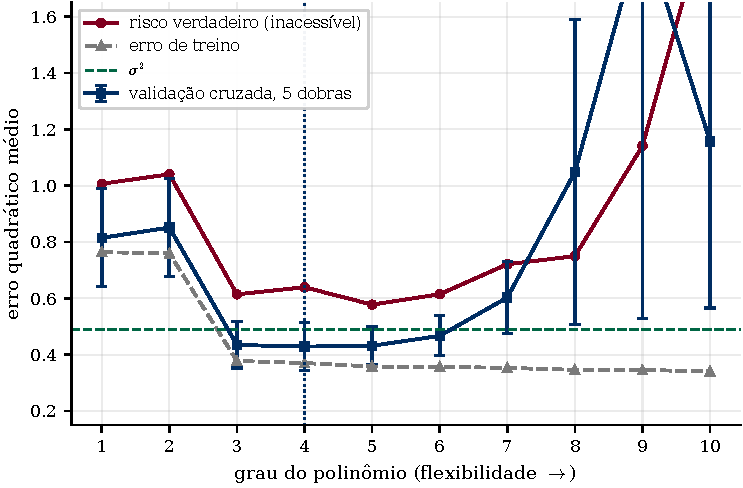
\includegraphics[width=0.78\textwidth]{../../recursos/figuras/03-cv-vs-risco.pdf}
  \caption{Validação cruzada de 5 dobras calculada sobre \emph{uma única} amostra de
  $n=50$, contra o risco verdadeiro e o erro de treino. As barras são de um
  erro-padrão. A CV reproduz a forma em ``U'' e localiza o mínimo no grau~4, contra
  o grau~5 do risco verdadeiro --- e, o mais importante, não se deixa enganar pelo
  erro de treino, que continua descendo. Note também as barras se abrindo à direita:
  a CV \emph{avisa} quando está insegura.}
  \label{fig:cvrisco}
\end{figure}

\begin{ideia}[o que a CV precisa acertar]
Repare que a curva azul não coincide com a vinho: a CV \emph{subestima} um pouco o
risco. Isso não é problema. Para \textbf{selecionar} um modelo, o que importa é
\emph{onde} está o mínimo, não o valor no mínimo. O [ISLP] faz essa observação
explicitamente: em três exemplos diferentes as curvas de CV ora subestimam, ora
superestimam o risco, mas todas identificam corretamente o nível de flexibilidade
certo. Se você quer \emph{reportar} o desempenho, aí sim precisa do valor --- e para
isso usa-se um conjunto de teste separado, ou CV aninhada.
\end{ideia}

\subsection{Viés, variância e a escolha de $k$}\label{sec:escolhak}
O argumento clássico para a escolha de $k$ é ele mesmo um balanço
viés--variância \emph{da estimativa do risco}:
\begin{itemize}[leftmargin=1.4cm]
  \item \textbf{$k$ grande (LOOCV):} cada $g_{-j}$ treina com $\approx n$ dados
        $\Rightarrow$ \emph{pouco viés}. Em contrapartida os $n$ modelos são quase
        idênticos entre si e suas predições, muito correlacionadas --- e a média de
        quantidades correlacionadas não se beneficia da lei dos grandes números como
        a de quantidades independentes. O argumento conclui: \emph{variância alta}.
  \item \textbf{$k$ pequeno (p.ex.\ $5$):} cada $g_{-j}$ treina com bem menos dados
        $\Rightarrow$ \emph{mais viés}, no sentido pessimista: o procedimento avaliado
        não é bem o que você vai usar no final. Em troca, as dobras são mais
        independentes.
\end{itemize}

\begin{ideia}[de onde vem o viés, e por que ele é sempre pessimista]
A Observação~\ref{obs:loo} já explica o viés do segundo item, e a explicação vale
para todo $k$. Com $k$ dobras de tamanho igual, cada $g_{-j}$ treina com $n-n/k$
observações, e o par $(\X_i,Y_i)$ de uma dobra continua sendo, para o modelo
ajustado sem ela, uma observação nova. Repetindo o cálculo de lá parcela por
parcela,
\[
  \E\big[\riscohat_{k\text{-CV}}\big] = \risco_{\,n-n/k},
  \qquad\text{quando você queria } \risco_n .
\]
Não há nada de misterioso no viés da validação cruzada: ele é o preço de avaliar um
procedimento treinado com \emph{menos dados} do que aquele que você vai usar no
fim. Com $k=10$ são 90\% da amostra e quase não se nota; com $k=2$, metade dela.

Duas consequências que vale guardar. A primeira é o \textbf{sinal}: como menos
dados costumam piorar o ajuste, $\risco_{\,n-n/k}\ge\risco_n$, e a validação
cruzada erra \emph{por cima}. Quando houver viés, ele será pessimista --- ao
contrário do erro de treino, que erra sempre por baixo. A segunda é que esse viés
não diz nada sobre a \emph{variância}: aquela depende de quanto as dobras se
parecem entre si, que é a outra metade do argumento clássico.
\end{ideia}

A Figura~\ref{fig:escolhak} mede o viés e o custo na nossa população.

\begin{figure}[htbp]
  \centering
  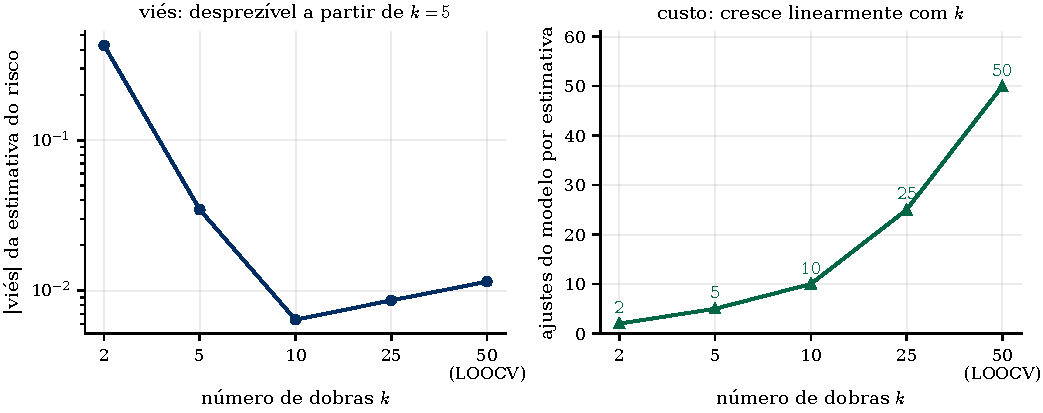
\includegraphics[width=\textwidth]{../../recursos/figuras/03-escolha-k.pdf}
  \caption{Estimativa do risco de um polinômio de grau~5 sobre $n=50$ pontos,
  repetida em 300 amostras independentes. À esquerda, o viés da estimativa (escala
  logarítmica): com $k=2$ ele é desastroso --- treinar com 25 pontos é coisa muito
  diferente de treinar com 50 --- e a partir de $k=5$ já é desprezível. À direita, o
  custo, que cresce linearmente: a LOOCV pede \emph{dez vezes} mais ajustes que
  $k=5$.}
  \label{fig:escolhak}
\end{figure}

\begin{atencao}[o que o experimento mostra]
O viés se comporta como previsto: cai de $0{,}43$ em $k=2$ para $0{,}006$ em $k=10$
--- treinar com metade dos dados é mesmo coisa muito diferente de treinar com todos,
e essa diferença some depressa. Some tão depressa que a conclusão prática se lê
direto do gráfico: de $k=5$ para frente não há praticamente nada a ganhar, e o
custo continua subindo linearmente. Daí $k=5$ ou $k=10$.
\end{atencao}

\begin{atencao}[A regra de ouro contra vazamento]
\textbf{Toda} etapa que ``aprende'' algo dos dados --- padronização, seleção de
variáveis, escolha de $\lambda$ --- deve ocorrer \emph{dentro} de cada dobra,
usando apenas o treino daquela dobra. Padronizar com a média/desvio de todo o
conjunto antes da CV é \emph{data leakage} e produz estimativas otimistas. (É por
isso que usamos \emph{pipelines}, Aula~07.)
\end{atencao}

\subsection{Selecionando hiperparâmetros}
O uso central: para cada valor de um hiperparâmetro $\theta$ (p.ex.\ $\lambda$ do
Lasso), calcule $\riscohat_{k\text{-CV}}(\theta)$ e escolha
$\widehat\theta=\argmin_\theta \riscohat_{k\text{-CV}}(\theta)$.

\begin{ideia}[o protocolo, em quatro passos]
Junte as peças e o procedimento inteiro fica assim:
\begin{enumerate}[leftmargin=1.6cm,nosep]
  \item \textbf{separe} o conjunto de teste (p.ex.\ 30\%) e guarde-o;
  \item \textbf{escolha} um ou mais bons candidatos por validação cruzada
        \emph{dentro do treino};
  \item \textbf{reajuste} o(s) candidato(s) em \emph{todo} o conjunto de
        treinamento --- as dobras serviram para escolher, não para entregar o
        modelo;
  \item \textbf{meça} o desempenho no conjunto de teste.
\end{enumerate}
O passo 3 é o que quase todo mundo esquece, e é ele que faz a CV valer a pena: o
modelo entregue usa \emph{todas} as observações de treino, não $k-1$ delas.
\end{ideia}

\begin{atencao}[Regra ``1-EP'']
Como $\riscohat_{k\text{-CV}}$ tem erro padrão, muitas vezes prefere-se a
\emph{regra de um erro-padrão}: escolher o modelo \emph{mais simples} cujo risco
estimado esteja a no máximo um erro-padrão do mínimo. Favorece parcimônia
(é o \texttt{lambda.1se} do \texttt{glmnet}). Na Figura~\ref{fig:cvrisco} ela
escolheria o grau~3 em vez do~4: como as barras de erro dos graus 3 a 6 se
sobrepõem, os dados não distinguem esses modelos, e nesse empate a regra manda ficar
com o mais simples.
\end{atencao}

\begin{atencao}[Validação \emph{aninhada}]
Se você usa CV para \emph{escolher} $\theta$ \emph{e} para \emph{reportar} o
desempenho, precisa de \textbf{CV aninhada}: um laço externo estima o desempenho,
um laço interno escolhe $\theta$. Usar a mesma CV para as duas coisas subestima o
risco --- é o mesmo pecado do erro de treino, um andar acima. O [AME] descreve a
versão com três conjuntos: \emph{treino} ajusta, \emph{validação} escolhe o
hiperparâmetro, e o \emph{teste}, tocado uma única vez no fim, estima o risco do
vencedor. Quanto mais modelos você comparar na validação, mais otimista ela fica ---
por isso o teste existe.
\end{atencao}

%==============================================================================
\section{O bootstrap}
%==============================================================================
A validação cruzada estima o \emph{risco}; o \textbf{bootstrap} estima a
\emph{incerteza} (variância, viés, intervalos) de praticamente qualquer
estatística $\widehat\theta$ calculada a partir dos dados.

\begin{ideia}
Não conhecemos $P$, mas temos a amostra. O bootstrap usa a \emph{distribuição
empírica} (reamostrar dos dados \emph{com reposição}) como substituta de $P$,
imitando o ato de coletar novas amostras.
\end{ideia}

\noindent\textbf{Algoritmo.} Para $b=1,\dots,B$:
\begin{enumerate}[leftmargin=1.6cm,nosep]
  \item sorteie $n$ observações \emph{com reposição} da amostra original (amostra
        bootstrap $\Dados^{*b}$);
  \item calcule a estatística $\widehat\theta^{*b}$ em $\Dados^{*b}$.
\end{enumerate}
A dispersão de $\{\widehat\theta^{*1},\dots,\widehat\theta^{*B}\}$ estima a
distribuição amostral de $\widehat\theta$; por exemplo,
$\widehat{\mathrm{EP}}(\widehat\theta)$ é o desvio-padrão dessas réplicas, e um
intervalo de confiança de 95\% pode ser dado pelos percentis $2{,}5\%$ e $97{,}5\%$.

\begin{exemplo}[O exemplo do {[ISLP]}: como dividir um investimento]
Você quer investir em dois ativos com retornos aleatórios $X$ e $Y$, pondo uma
fração $\alpha$ em $X$ e $1-\alpha$ em $Y$. Para minimizar o risco da carteira,
$\Var(\alpha X+(1-\alpha)Y)$, a fração ótima é
\[
  \alpha = \frac{\sigma_Y^2-\sigma_{XY}}{\sigma_X^2+\sigma_Y^2-2\sigma_{XY}} .
\]
Na prática você não conhece $\sigma_X^2$, $\sigma_Y^2$ e $\sigma_{XY}$: estima-os
dos dados e obtém $\widehat\alpha$. Qual o erro-padrão de $\widehat\alpha$? Boa
sorte tentando derivá-lo analiticamente --- é uma razão de estimativas
correlacionadas. Com bootstrap são cinco linhas de código: reamostre, recalcule
$\widehat\alpha^{*b}$, tome o desvio-padrão. É aí que está a força do método:
funciona para estatísticas cuja distribuição amostral ninguém sabe escrever.
\end{exemplo}

\begin{observacao}
Cada amostra bootstrap deixa de fora, em média, $\approx 1/e \approx 37\%$ das
observações originais (as \emph{out-of-bag}). A conta: uma observação específica
escapa de um sorteio com probabilidade $1-1/n$, e de $n$ sorteios com probabilidade
$(1-1/n)^n \to e^{-1} \approx 0{,}368$. Essa ideia reaparece no \emph{bagging} e nas
florestas aleatórias (Aula~06), onde as observações OOB dão uma estimativa de risco
``de graça'' --- sem separar dados nem rodar CV.
\end{observacao}

%==============================================================================
\section{Prática em Python}
%==============================================================================
\begin{lstlisting}
from sklearn.model_selection import (train_test_split, cross_val_score, KFold,
                                     GridSearchCV)
from sklearn.pipeline import make_pipeline
from sklearn.preprocessing import StandardScaler
from sklearn.linear_model import Ridge
from sklearn.metrics import mean_squared_error

# 0. O PRIMEIRO passo e separar o teste. Dobra nenhuma vai toca-lo.
X_tr, X_te, y_tr, y_te = train_test_split(X, y, test_size=0.3, random_state=0)

modelo = make_pipeline(StandardScaler(), Ridge(alpha=1.0))
dobras = KFold(5, shuffle=True, random_state=0)

# 1. CV DENTRO DO TREINO, para estimar o risco de UM procedimento
#    (MSE -> negativo no sklearn)
scores = cross_val_score(modelo, X_tr, y_tr, cv=dobras,
                         scoring="neg_mean_squared_error")
print("risco estimado:", -scores.mean(), "+/-", scores.std())

# 2. Selecionar o hiperparametro lambda (=alpha) por CV, SEM vazamento
#    (o StandardScaler e reajustado dentro de cada dobra)
grade = {"ridge__alpha": [0.01, 0.1, 1, 10, 100]}
busca = GridSearchCV(modelo, grade, cv=dobras, scoring="neg_mean_squared_error")
busca.fit(X_tr, y_tr)                 # o teste continua guardado
print("melhor alpha:", busca.best_params_)

# 3. O vencedor ja saiu reajustado em TODO o treino (refit=True, o padrao).
#    So agora o teste e tocado, uma unica vez.
print("EQM no teste:", mean_squared_error(y_te, busca.predict(X_te)))
\end{lstlisting}

\begin{atencao}
Três coisas a reparar nesse trecho. Primeira: as funções de \emph{score} seguem a
convenção ``maior é melhor'', então o EQM aparece negado
(\texttt{neg\_mean\_squared\_error}) --- daí o sinal de menos ao imprimir. Segunda:
o \texttt{KFold} está construído explicitamente, e não passado como
\texttt{cv=5} --- assim é passado \texttt{shuffle=True}, sem o qual as dobras saem
\emph{na ordem do arquivo}, com o problema descrito no início da aula. Terceira: o
\texttt{X\_te} aparece uma única vez no trecho inteiro, na última linha. Se ele
aparecer antes disso, alguma coisa está errada.
\end{atencao}

O notebook \texttt{Aula prática 03} refaz tudo isto: implementa as $k$ dobras à mão,
confere o atalho do LOOCV, roda o protocolo de quatro passos numa população em que
a resposta é conhecida, e fecha escolhendo o $\lambda$ de uma Ridge no
\texttt{superconductivity.csv}.

%==============================================================================
\section*{Resumo}
%==============================================================================
\begin{itemize}[leftmargin=1.4cm]
  \item O erro de treino é otimista; estimar o risco exige dados \emph{não}
        usados no ajuste.
  \item \emph{Data splitting}: simples, mas desperdiça dados e é instável.
  \item \emph{LOOCV} \eqref{eq:loocv}: quase não-viesado; atalho fechado para
        modelos lineares (Prop.~\ref{prop:loo}).
  \item \emph{$k$-dobras} \eqref{eq:kfold}: usa toda a amostra
        (Fig.~\ref{fig:kfold}); $k=5$ ou $10$ bastam --- além disso só cresce o
        custo (Fig.~\ref{fig:escolhak}).
  \item A CV pode errar o \emph{nível} do risco e ainda assim acertar \emph{onde}
        está o mínimo (Fig.~\ref{fig:cvrisco}) --- e é isso que a seleção de
        modelos precisa.
  \item Use CV para escolher \emph{tuning parameters}; cuidado com \emph{vazamento}
        (faça tudo dentro da dobra) e com CV aninhada para reportar desempenho.
  \item \emph{Bootstrap}: reamostragem com reposição para medir incerteza de
        estimativas; conecta com OOB e \emph{bagging}.
\end{itemize}

\paragraph{Leitura recomendada.} [AME] §1.4 (função de risco e Teorema~1), §1.5.1
(\emph{data splitting}, validação cruzada, a Observação~1.5 sobre o LOOCV
não-viesado e o intervalo de confiança para o risco). [ISLP] Capítulo~5: §5.1
(validação cruzada --- vale muito olhar as Figuras~5.6 e~5.8, que são a versão deles
da nossa Figura~\ref{fig:cvrisco}), §5.1.4 (o argumento viés--variância para a
escolha de $k$) e §5.2 (\emph{bootstrap}, com o exemplo do investimento).

\paragraph{Para praticar.} \texttt{Lista teorica 03.pdf} (teórica, com gabarito) e \texttt{Lista prática 03.ipynb} (prática, para completar as lacunas), nesta mesma pasta.

\end{document}
